%! TEX root = main.tex

%/========== Acrobot ==========/%

\chapter{Application of VNHCs: The Acrobot}\label{ch:acrobot}
\section{Motivation}
The acrobot is a two-link pendulum, actuated at the center joint (as in Figure
\ref{fig:acrobot-model}). 
Since its first description in 1990
\cite{nonlinear_controllers_nonintegrable_acrobot}, the acrobot has become a
benchmark problem in control theory; 
it is an underactuated mechanical system which produces complex nonlinear motion
from an easy-to-describe model.
The acrobot models a gymnast on a bar, since it represents a torso (top link)
and legs (bottom link) with motion generated by the swinging of the legs at the
hips. 
It is also one of the simplest models for a biped walking robot
\cite{toward_framework_biped_locomotion}.

\begin{figure}
    \centering
    \includestandalone[width=0.7\textwidth]{images/acrobot_model}
    \caption{The general acrobot model, represented by two weighted rods
    differing in both length and mass.}%
    \label{fig:acrobot-model}
\end{figure}

Controlling the acrobot is a nontrivial task because it is not feedback
linearizable \cite{nonlinear_controllers_nonintegrable_acrobot}. 
Several researchers have studied the swing-up problem of driving the acrobot to
its equilibrium point above the bar using partial feedback linearization
\cite{swingup_problem_acrobot}, energy-based control
\cite{swingup_acrobot_pendulum, swingup_acrobot_energy}, and through studying
human motion \cite{swingup_giant_acrobot, motion_control_gymnastic_skill}.

In gymnastics terminology, a ``giant" is the motion a gymnast performs to
achieve full rotations around the bar \cite{usagym_giant}. 
We are interested in using VNHCs to generate giant motion, with the aim of
stabilizing desired energy levels.
The control of giant motion for the acrobot has been studied in
\cite{energy_pumping_robotic_swinging, swingup_giant_acrobot}, 
and some authors have used virtual holonomic constraints to achieve this
behaviour
\cite{dynamical_servo_acrobot_vc, control_giant_two_link_gymnastic_robot,
xingbo_thesis}. 
However, these controllers are neither intuitive nor easy to
design:
\cite{control_giant_two_link_gymnastic_robot} defines a constraint by inverting
a trajectory in time onto the state space; 
\cite{dynamical_servo_acrobot_vc} requires a cascade controller to stabilize
both a constraint and a desired limit cycle in the state space; 
and \cite{xingbo_thesis} enforces the giant by adding an extra state to estimate
velocity, which increases the dimensionality of the problem in a crude
approach to using VNHCs.

In this chapter we will design a physically-intuitive VNHC which generates giant
motion and prove the acrobot gains energy. 
In the process of completing this proof, we will arrive at a promising method
which might one day be useful for generating energy-injecting VNHCs on arbitrary
mechanical systems.

\section{Dynamics of the Acrobot}
Suppose we are given an acrobot as in Figure \ref{fig:acrobot-model} modelling a
gymnast hanging on a horizontal bar, where the ``torso" has moment of
inertia \(J_u\) and the ``leg" has moment of inertia \(J_a\) (each with respect
to their own center of mass).
Let \(q_u \in \Sone\) be the shoulder angle and \(q_a \in \Sone\) 
be the hip angle, where only \(q_a\) is actuated. 
Collecting them together provides the configuration
\(q = (q_u,q_a) \in \Sone \times \Sone\). 
The acrobot has inertia matrix \(D\), potential function \(P\) (with respect to
the horizontal bar), and input matrix \(B\)  given as
follows \cite{xingbo_thesis}:
\begin{align}\label{eqn:general-acrobot-inertia}
    D(q) &= \begin{bmatrix}
      m_al_u^2 + 2m_a\cos(q_a)l_u l_{c_a} + m_al_{c_a}^2 + m_ul_{c_u}^2 + J_u + J_a &
      m_al_{c_a}^2 + m_al_ul_{c_a}\cos(q_a) + J_a \\
      m_al_{c_a}^2 + m_al_ul_{c_a}\cos(q_a) + J_a &
      m_al_{c_a}^2 + J_a
    \end{bmatrix} 
    , \\
    \label{eqn:general-acrobot-potential}
    P(q) &= g\left(m_al_{c_a}(1 - \cos(q_u+q_a)) + 
        (m_al_u + m_ul_{c_u})(1-\cos(q_u))\right) 
    , \\
    B(q) &= \begin{bmatrix} 0 \\ 1 \end{bmatrix}
    .
\end{align}

While this is the most general representation of an acrobot, the dynamics
are unwieldy.
To make rigorous analysis of these dynamics more tractable, we begin by assuming
the acrobot is comprised of two massless rods of equal length \(l\), with equal
point masses \(m\) at the tips.
We call this a \textit{simple} acrobot, which is displayed in Figure
\ref{fig:simple-acrobot-model}.
We will also ignore any frictional forces at both the hip and shoulder joints. 
Finally, it is important to note that a real gymnast cannot swing their legs in
full circles, though they are usually flexible enough to raise them parallel to
the floor; 
for this reason, we assume that \(q_a \in [-Q_a, Q_a]\) where 
\(Q_a \in [\frac{\pi}{2}, \pi[\). 

\begin{figure}
    \centering
    \includestandalone[width=0.7\textwidth]{images/simple_acrobot_model}
    \caption{A simple acrobot has massless rods of equal length \(l\) and 
    equal masses \(m\) at the tips.}
    \label{fig:simple-acrobot-model}
\end{figure}

Since we are now working with a simple acrobot, 
we have \(l_{c_u} = l_{c_a} = l_u = l_a = l\) and
\(m_u = m_a = m\). 
On top of this, the moments of inertia \(J_u\) and \(J_a\) of the rods vanish.
Reducing
~\eqref{eqn:general-acrobot-inertia}-\ref{eqn:general-acrobot-potential}
yields the simplified inertia matrix \(D_s\) and potential function \(P_s\),
where
\begin{align}
    D_s(q) &= \begin{bmatrix}
        ml^2\left(3+2\cos(q_a)\right) & 
        ml^2\left(1+\cos(q_a)\right) \\
        ml^2\left(1+\cos(q_a)\right) &
        ml^2
    \end{bmatrix} 
    , \\
    P_s(q) &= -mgl\left(2\cos(q_u)+\cos(q_u+q_a)\right)
    .
\end{align}
\begin{notation}
    For shorthand, we write \(c_u := \cos(q_u)\), \(c_a := \cos(q_a)\), and 
    \(c_{ua} := \cos(q_u + q_a)\). Likewise, \(s_u := \sin(q_u)\), 
    \(s_a := \sin(q_a)\), and \(s_{ua} := \sin(q_u + q_a)\).
\end{notation}

Defining \(M(q) := D_s(q)\) and \(V(q) := P_s(q)\), we find the conjugate of momenta 
is \(p = (p_u, p_a) = M(q)\dot{q}\).
The dynamics in \((q,p)\) coordinates are given by
\begin{align}\label{eqn:acrobot-hamiltonian}
    \mathcal{H}(q,p) &= \frac{1}{2}p\tpose \Minv(q) p -
    mgl\left(2 c_u + c_{ua}\right)
    , \\
     &\begin{cases}
        \dot{q} = \Minv(q) p \\
        \dot{p}_u = -mgl\left(2s_u + s_{ua}\right) \\
        \dot{p}_a =-\frac{1}{2}p\tpose \nabla_{q_a}\Minv(q) p
        - mgl s_{ua} + \tau,
    \end{cases} \nonumber
\end{align}
where the inverse inertia matrix is
\begin{equation}\label{eqn:Minv}
    \Minv(q) = \frac{1}{ml^2\left(2-c_a^2\right)}
    \begin{bmatrix}
        1 &
        -\left(1+c_a\right) \\
        -\left(1+c_a\right) &
        3+2c_a
    \end{bmatrix}
    .
\end{equation}
The control input is a force \(\tau \in \R\) affecting only the dynamics of
\(p_a\), representing a torque acting on the hip joint.
This means \((q,p)\) are simply actuated coordinates inside the phase space
\(\mathcal{Q} \times \mathcal{P}\) where
\(\mathcal{Q} = \mathcal{Q}_u \times \mathcal{Q}_a 
:= \Sone \times \Sone\), and
\(\mathcal{P} = \mathcal{P}_u \times \mathcal{P}_a
:= \R \times \R\).
This allows us to apply the theory of VNHCs from Chapter
\ref{ch:vnhcs}.

Let us define the VNHC \(h(q,p) = q_a - f(q_u,p_u)\) of order 1, where
\(f \in C^2\left(\mathcal{Q}_u \times \mathcal{P}_u; \mathcal{Q}_a\right)\).
Since \(\nabla_{q_u}\Minv(q) = \Zmat{2\times 2}\),
Theorem \ref{thm:vnhc-regularity} tells us that this VNHC will be regular
when the regularity matrix
\[
    dh_q \Minv(q) \begin{bmatrix}0 \\ 1 \end{bmatrix}
    ,
\]
is of full rank \(1\) on the constraint manifold \(\Gamma\).
Given that
\(dh_q = \begin{bmatrix} -\partial_{q_u} f & 1 \end{bmatrix}\),
the regularity matrix evaluates to the scalar equation
\begin{equation}\label{eqn:regularity-matrix-acrobot}
    \frac{(1+c_a)\partial_{q_u}f(q_u,p_u) + (3+2c_a)}{ml^2(2-c_a^2)}
    .
\end{equation}
This is full rank if and only if the numerator does not
change sign.
The following proposition provides a sufficient condition for regularity.

\begin{prop}\label{prop:acrobot-fpu-regular}
    A relation \(h(q,p) = q_a - f(p_u) = 0\) for ~\eqref{eqn:acrobot-hamiltonian} 
    with \(f \in C^2\left(\mathcal{P}_u; \mathcal{Q}_a\right)\) is a regular
    VNHC of order 1.
\end{prop}
\begin{proof}
    Since \(\partial_{q_u} f = 0\), the regularity equation
    ~\eqref{eqn:regularity-matrix-acrobot} is strictly positive for all values
    of \(q_a\), and hence is full rank everywhere on the constraint manifold.
    By Theorem \ref{thm:vnhc-regularity}, \(h\) is a regular VNHC of order 1.
\end{proof}
Proposition \ref{prop:acrobot-fpu-regular} will be useful later, as we will not
need to check regularity if we design a function of the unactuated momentum. 

The acrobot is noticeably more complex than the VLP, as
the dynamics of \((q_u,p_u)\) and \((q_a,p_a)\) are coupled through \(\Minv(q)\).
Because of this, the constrained dynamics of an arbitrary VNHC may not be easy
to write out.
In the rest of this chapter, our goal is to design the function \(f(q_u,p_u)\)
based on the natural human motion of a gymnast, with one caveat: 
we must be able to prove the constrained dynamics will inject energy into the
acrobot.

\section{Previous Constraint Approaches}
% TODO: Give Xingbo's intuition, abstract away to qa = sin(theta) constraint
% based on VLP but show it doesn't work well in our framework
% TODO: Describe Xingbo's results and observe that his results were similar to a VNHC
% except they used VHC tools. We will modify his approach to use VNHCs and prove
% rigorously that we can stabilize any energy level set on the acrobot.
Let us examine some of the existing approaches to generating giant motion for
the acrobot, since these may be viable candidates on which to base a VNHC.

One initial approach to controlling the acrobot is to model it as a
variable-length pendulum by collapsing the two rods and masses into one
equivalent center of mass (ECM), as in Figure \ref{fig:acrobot-ecm}.
This seems a reasonable model reduction, since the length from the pivot to the
ECM changes depending on the angle \(q_a\) of the leg.
Indeed, \citet{swingup_giant_acrobot} use this approach to design a trajectory
for the ECM, then determine which leg angles \(q_a(t)\) are required to generate
that trajectory.
Following in their footsteps, we might consider using the results
from Chapter \ref{ch:vlp} to find the leg angles that allow the ECM to gain
energy. 
Then we could apply Theorem \ref{thm:vlp-energy-stabilization} to prove
the acrobot is gaining energy.
\begin{figure}
    \centering
    \includestandalone[width=0.5\textwidth]{images/acrobot_ecm}
    \caption{A simple acrobot modelled as a VLP with equivalent center of mass \(2m\). 
        The length of the VLP changes according to \(q_a\).}
    \label{fig:acrobot-ecm}
\end{figure}

Unfortunately, the VLP is not a true representation of the acrobot.
The effective length of the ECM is 
\[
    l_e(q_a) := l\sqrt{\frac{5}{4} + c_a}
    ,
\]
and its effective angle is
\[
    q_e := \arctan_2\left(s_u + \frac{1}{2}s_{ua}, -c_u - \frac{1}{2}c_{ua}\right)
    .
\]
There are two important notes to consider based on these equations. 
First, Figure \ref{fig:acrobot-vlp-symmetry} shows that for each pose of the
VLP representation, there are two configurations
of the acrobot which give the same effective length and angle.
This means the acrobot and the VLP are not equivalent representations;
designing a VNHC that injects energy using the ECM may not produce human-like
leg motion on the acrobot.

Second, if we were to compute the conjugate of momenta
\(p_{l_e}\) to \(l_e\) and \(p_e\) to \(q_e\), we would see the torque input
\(\tau\) appearing in both of their dynamic equations.
In the VLP model from Chapter \ref{ch:vlp}, the control input only
affects the dynamics of the length variable.
If we want to design a VNHC for this system, we cannot use any of the results
from Chapter \ref{ch:vlp} because the VLP models do not match.

\begin{figure}
    \centering
    \includestandalone[width=0.3\textwidth]{images/acrobot_vlp_symmetry}
    \caption{The equivalent center of mass of the acrobot generally has two configurations
        which correspond to the same effective length and angle. These
        configurations are symmetric about the line connecting the pivot to the
        ECM.}
    \label{fig:acrobot-vlp-symmetry}
\end{figure}

Since we cannot apply the results of Chapter \ref{ch:vlp} to simplify the proof
of energy injection, and the resulting ECM motion may not even produce
realistic leg motion, this model reduction is ineffective for our purposes. 

Let us turn next to the thesis of \citet{xingbo_thesis}, who designs a VHC to enforce a
so-called ``tap" motion with the purpose of injecting energy into the acrobot. 
First, he defines a compensator variable \(s\) which tracks \(\dot{q}_u\), so
that he can use the theory of VHCs with the extended configuration 
\((q_u,q_a,s)\).
He then finds \(h_1, h_2 \in \R_{>0}\) to define the
normalized radius \(\rho\) and normalized angle \(\xi\) in the
\((q_u, s)\)-plane.
These normalized variables are given by
\begin{align*}
    \rho &:= \sqrt{h_1 q_u^2 + h_2 s^2}
    , \\
    \xi &:= \arctan_2(h_2 s, h_1 q_u)
    . 
\end{align*}
He then sets the VHC to be \(h(q) = q_a - f_\text{rad}(\rho)f_\text{ang}(\xi)\)
with the control parameters \(\bar{q}_u\) and \(\rho_0\), where
\begin{align}
    \label{eqn:xingbo-frad}
    f_\text{rad}(\rho) &:= \tanh^2(\rho/\rho_0)
    , \\
    \label{eqn:xingbo-fang}
    f_\text{ang}(\xi) &:= 
    \begin{cases}
        0 & -\pi < \xi \leq 0 \\
        \bar{q}_u \exp\left(1 - \frac{1}{1-(\frac{4\xi}{\pi} - 1)^2}\right) 
          & 0 < \xi \leq \frac{\pi}{2} \\
        0 & \frac{\pi}{2} < \xi \leq \pi
        .
    \end{cases}
\end{align}

While this constraint shows promising experimental results and it accurately
emulates true human motion, \citeauthor{xingbo_thesis}
does not provide analytical proof that the acrobot will gain energy.
His lack of analysis is tied to the fact that the constrained
dynamics are incredibly complicated.
In fact, just showing the constraint is regular is a challenging task.
While we could very easily convert his VHC into a VNHC by replacing \(s\) with
\(p_u\), we would run into the same problem. 
Since we want our constraint to \textit{provably} inject energy, we must forgo
this type of constraint in favour of something less complex.

\section{The Acrobot Constraint}
% TODO: Give the constraint, state the theorem, and show the outline of the
% proof (both as a sketch and in a figure)
One may be tempted to design a constraint of the form \(q_a = \bar{q}_a\sin(\theta)\) 
with \(\theta := \arctan_2(p_u,q_u)\), since a similar approach 
was so effective for the VLP in Chapter \ref{ch:vlp}.
Unfortunately, this constraint is not regular, and it is difficult to find any
VNHC of the form \(q_a = f(\theta)\) where regularity can be proven easily.
Instead, we will develop a constraint \(h(q,p) = q_a - f(p_u)\) because these
constraints are always regular (as per Proposition \ref{prop:acrobot-fpu-regular}). 
 
To design this constraint, let us begin (perhaps unexpectedly) by examining a person on
a seated swing.
The person extends their legs when the swing moves forwards, and retracts their
legs when the swing moves backwards.
As the swing gains speed, the person leans their body back while
extending their legs.
This allows them to bring their legs higher, shortening the distance
from their center of mass to the pivot and adding more energy to the swing.
When the swing moves backward, they sit up and fully retract their legs
underneath them \cite{how_to_pump_a_swing}.

Now imagine the person's torso is affixed to the swing's rope so that they are
always upright. 
Imagine further that the swing has no seat at all, allowing the person to extend
their legs beneath them. 
This position is identical to that of a gymnast on a bar, which is why we can
use leg motion from the seated swing to design a controller for the acrobot.

The acrobot's legs are rigid rods which cannot retract; so we emulate the person
on a swing by pivoting the legs toward the direction of motion. 
To account for how a person leans back at higher speeds, the legs should pivot to an
angle proportional to the swing's speed.
Since the direction of motion is entirely determined by \(p_u\), 
one such VNHC which emulates this process is \(q_a = \bar{q}_a\arctan( I p_u)\),
displayed in Figure \ref{fig:qa-arctan}.
Here, \(\bar{q}_a \in ]0,\frac{2 Q_a}{\pi}]\) and \(I \in \R_{>0}\) is a fixed
control parameter.

This constraint does not perfectly recreate giant motion, during which
the gymnast's legs are almost completely extended -- it instead pivots the legs
partially during rotations.
However, the behaviour looks similar enough that the constraint should provide a
decent foundation for injecting energy into the acrobot.
It is for this reason that we choose our acrobot's constraint to be
\begin{equation}\label{eqn:acrobot-constraint}
    h(q,p) = q_a - \bar{q}_a \arctan(I p_u)
    .
\end{equation}

\begin{figure}
    \centering
    \includestandalone[width=0.5\textwidth]{images/qa_arctan}
    \caption{The acrobot constraint \(q_a = \bar{q}_a \arctan(I p_u)\).}
    \label{fig:qa-arctan}
\end{figure}

Let us now compute the constrained dynamics under
~\eqref{eqn:acrobot-constraint}.
Note that \(dh_q = \begin{bmatrix}0 & 1\end{bmatrix}\), while
\[
    dh_{p_u} = \frac{-\bar{q}_a I}{1 + I^2 p_u^2}
    .
\]
Inserting these to ~\eqref{eqn:g-qupu}, we get the solution for \(p_a\) on the
constraint manifold:
\[
    p_a(q_u,p_u) = \frac{
        (1+c_a)(1+I^2 p_u^2)p_u - m^2gl^3\bar{q}_a I (2-c_a^2)(2s_u + s_{ua})
    }{ml^2(3+2c_a)(1+I^2 p_u^2)}
    .
\]
The dynamics for \(p_u\) do not contain \(p_a\), so they remain unchanged.
The constrained dynamics for \(q_u\) are given by 
\begin{equation*}
    \dot{q}_u = e_1\tpose \Minv(q) \begin{bmatrix}
                    p_u \\ p_a(q_u,p_u)
                \end{bmatrix} %\\
    ,
\end{equation*}
which can be simplified into 
\begin{equation*}
    \dot{q_u} = \frac{(1+I^2 p_u^2)p_u + m^2gl^3\bar{q}_a I(2s_u + s_{ua})(1+c_a) }{ml^2(1+I^2 p_u^2)(3+2c_a)}
    .
\end{equation*}
Hence, the constrained dynamics for the acrobot under
~\eqref{eqn:acrobot-constraint} are
\begin{equation}\label{eqn:acrobot-constrained-dynamics}
\left.\begin{cases}
    \dot{q}_u &= \frac{(1+I^2 p_u^2)p_u + m^2gl^3\bar{q}_a I(2s_u + s_{ua})(1+c_a) }
            {ml^2(1+I^2 p_u^2)(3+2c_a)}
        \\
    \dot{p}_u &= - m g l (2s_u + s_{ua})
    .
    \end{cases} \right|_{q_a = \bar{q}_a\arctan(Ip_u)}
\end{equation}

These dynamics do not always gain energy -- we need certain conditions on our
control parameter \(I\) to guarantee this is true.

\begin{thm}\label{thm:acrobot-energy-stabilization}
    Consider the simple acrobot ~\eqref{eqn:acrobot-hamiltonian} constrained by
    the VNHC ~\eqref{eqn:acrobot-constraint}, whose
    constraint manifold is \(\Gamma \simeq \SxR\).
    Let 
    \[
        E(q_u,p_u) := \frac{p_u^2}{10ml^2} + 3(1 - \cos(q_u))
        ,
    \]
    be the energy of the simple pendulum obtained by setting \(I = 0\).
\begin{enumerate}
    \item For all \(\epsilon > 0\), there exists \(I > 0\) small enough that 
    ~\eqref{eqn:acrobot-constraint} injects energy into the acrobot on the set
    \[
        \mathcal{O}_\epsilon := \left\{(q_u,p_u) \in \Gamma 
        \mid E(\epsilon,0) < E(q_u,p_u) < E(\pi,0) \right\}
        .
    \]
    If instead \(I < 0\), the VNHC dissipates energy on \(\mathcal{O}_\epsilon\).
\item Define \(b : \SxR_{> 0} \rightarrow \R\) by
    \[
        b(\beta,\rho_0) := 
        \frac{5m^2 g l^3 \bar{q}_a \left(
            m^2gl^3\left(18s_\beta^2 + 30c_\beta(1 - c_\beta)\right)
            - c_\beta\rho_0^2
        \right)}{
        |\rho_0|\sqrt{\rho_0^2 - 30m^2gl^3(1 - c_\beta)}
        }
        ,
    \]
    and fix \(\bar{\rho} > \sqrt{60m^2gl^3}\).
    Suppose \(\int \limits_{0}^{2\pi} b(\sigma,\rho_0)d\sigma > 0\) for all 
    \(\rho_0 \in \, \left]\sqrt{60m^2gl^3}, \bar{\rho}\right[\).
    Then there exists \(I > 0\) small enough that
    ~\eqref{eqn:acrobot-constraint} injects energy into the acrobot on
    \[
        \Omega := \left\{(q_u,p_u) \in \Gamma 
            \mid E(q_u,p_u) < E(0,\bar{\rho})\right\}
        .
    \]
    If instead \(I < 0\), the VNHC dissipates energy on \(\Omega\).
\end{enumerate}
\end{thm}
%\footnotetext{In fact, we can be more precise than this. 
%    Letting \(\epsilon > 0\), we need 
%    \(I \leq \min\left\{I_1(\epsilon),I_2\}\) where
%    \(I_1(\epsilon) = \frac{\tan(\epsilon)}{(\pi-\epsilon)}
%    \left(\frac{m^2gl^3(\cos(\epsilon)-2\sin(\epsilon))}{\pi-\epsilon}
%    \left(\frac{2\bar{q}_a\tan(\epsilon)}{(1+\tan(\epsilon)^2)(\pi-\epsilon)}+5\right) 
%    \right)^{-1/2}\)
%    and \(I_2 = \sqrt{\frac{3}{10 m^2gl^3\bar{q}_a^2}}\).
%    See Apendix \ref{apx:I-bounds} for details.
%}
The region \(\mathcal{O}\) is the oscillation domain of the simple pendulum
obtained by setting \(q_a = 0\);
\(\Omega\) includes \(\mathcal{O}\), alongside all rotations of this 
pendulum with momentum less than \(\bar{\mu}\). 
Hence, the first result of Theorem \ref{thm:acrobot-energy-stabilization} states
that the acrobot will gain enough energy to begin performing giant motion;
the second result guarantees can achieve giants with momentum
\(|p_u| < \bar{\mu}\).

Unfortunately, the energy-based proof used in Chapter \ref{ch:vlp} does not
readily transfer to the acrobot -- there is no obvious Lyapunov function for
this constrained system.
Proving Theorem \ref{thm:acrobot-energy-stabilization} requires an intelligent
change of coordinates and the use of perturbation theory from
\cite{khalil_nonlinear}.
The full proof is given in Chapter \ref{sec:acrobot-proof}, so 
we conclude this section with a high level sketch of the proof.

There is a suitable change of coordinates into a pseudo-radius 
\(\mu \in \R_{>0}\) and pseudo-angle \(\alpha \in \Sone\) on the
\((q_u,p_u)\)-plane.
These coordinates have the property that \(\dot{\alpha} > 0\) when
\(I\) is small enough.
Perturbation theory shows that (for possibly smaller \(I\)) the radius \(\mu\)
increases on average along \(\alpha\).
Hence, orbits in the \((q_u,p_u)\)-plane spiral away from the origin, 
which means the acrobot is gaining energy.
 
\section{Proving the Acrobot Gains Energy}\label{sec:acrobot-proof}
% TODO: Prove this in sections
% TODO: You don't have to use the proof of theta_dot being positive. Stick to
% Manfredi's proof, and when you say "for I small enough" put in a footnote that
% says "in fact, we can be more precise and set bounds for I given as I <
% min{...}. See appendix for more detail."
% Then, we can have an appendix where we derive the bounds on I so that
% theta_dot is always positive. This will help the reader keep track and not
% bother them too much.
Proving Theorem \ref{thm:acrobot-energy-stabilization} is not a simple task.
In an effort to make the proof as clear as possible, we will break it down into
the following segments:
\begin{enumerate}
    \item Background on perturbation theory.
    \item Perturbation analysis for oscillations.
    \item Energy gain for oscillations.
    \item Perturbation analysis for rotations.
    \item Energy gain for rotations.
\end{enumerate}

When \(I = 0\), the constrained acrobot behaves like a single
pendulum with masses at a distance \(l\) and \(2l\) from the pivot 
(Figure \ref{fig:acrobot-I0}) whose energy
\begin{equation}\label{eqn:acrobot-nominal-E}
    E(q_u,p_u) = \frac{p_u^2}{10ml^2} + 3(1 - \cos(q_u))
    ,
\end{equation}
is conserved.
Level sets of \(E\) are ellipses when \(E(q_u,p_u) < E(\pi,0)\), which we call
``oscillations"; and they are open curves when \(E(q_u,p_u) > E(\pi,0)\), which we call
``rotations". 
Examples of these can be seen in Figure \ref{fig:pendulum-level-sets}.

\begin{figure}
    \centering
    \begin{subfigure}[t]{0.45\textwidth}
        % TODO: figure of acrobot with I = 0
        %\includestandalone[]{images/acrobot_I0}
        \caption{The simple pendulum with two masses.}
        \label{fig:acrobot-I0}
    \end{subfigure}
    \hfill
    \begin{subfigure}[t]{0.45\textwidth}
        % TODO: figure showing oscillations and rotations as level curves of E
        %\includestandalone[]{images/pendulum_level_sets}
        \caption{Level sets of the pendulum energy function.
            The red ellipse represents oscillations while the purple curve
            represents rotations.}
        \label{fig:pendulum-level-sets}
    \end{subfigure}
    \caption{Our constrained acrobot is a simple pendulum when \(I = 0\).}
\end{figure}

Using a method developed by \citet{dynamic_vhcs_stabilize_closed_orbits},
we can find a change of coordinates \((q_u,p_u) \to (\alpha, \mu)\) with the
following properties:
\begin{itemize}
    \item The energy of oscillation in \((\alpha,\mu)\) coordinates is 
        uniquely defined by \(\mu\), which remains constant along oscillations
        of the simple pendulum.
    \item \(\alpha\) is a pseudo-angle living in \(\Sone\) which is
        always increasing.
\end{itemize}
Once we have these coordinates in hand, we can use perturbation theory to prove
that \(\mu\) increases on average for the acrobot when \(I\) is small enough.
Likewise, we will find a second set of coordinates \((\beta, \rho)\) where
\(\beta \in \Sone\) is always increasing, \(\rho\) is constant along
rotations of the simple pendulum, and \(\rho\) increases for the acrobot when
\(I\) is small enough.
Putting these together, we will show the acrobot is gaining energy.

\subsection*{Background on Perturbation Theory}
Nonlinear systems like the acrobot are difficult (or impossible) to solve
analytically.
Perturbation theory allows one to understand the behaviour of the nonlinear system
by studying a simpler nominal system. 
Solutions of the nonlinear system can often be approximated by taking a Taylor
expansion around this nominal system.

\citet{khalil_nonlinear} considers a system of the form

\begin{equation}\label{eqn:khalil-setup}
    \begin{cases}
        \dot{x} = f(t,x,I), \\
        x(t_0) = \eta(I),
    \end{cases}
\end{equation}
where 
\(f : [t_0,t_1] \times D \times [-I_0,I_0] \rightarrow \R^n\) is smooth
\footnote{Khalil actually considers \(f(t,x,\epsilon)\) which is ``sufficiently
    smooth". We replace \(\epsilon\) with \(I\) and assume smoothness to
    more easily connect his theory to the acrobot constraint.}.
In the context of the acrobot, \(x\) is the set of coordinates which make
our analysis convenient;
\(I\) is a parameter of the system;
the function \(f\) is the constrained dynamics in \(x\)-coordinates;
and \(\eta(I) \equiv \eta_0\) is a constant initial condition.

Setting \(I = 0\) we get the nominal system
\begin{equation}\label{eqn:khalil-perturbation-nominal}
    \begin{cases}
        \dot{x}_0 = f(t,x,0) ,\\
        x_0(t_0) = \eta_0 ,
    \end{cases}
\end{equation}
which we need to solve for the explicit solution \(x_0(t,\eta_0)\) on \([t_0,t_1]\).
One can use this to compute the solution \(x_1(t,\eta_0)\) of
\begin{equation}\label{eqn:khalil-perturbation-firstorder}
    \begin{cases}
        \dot{x}_1 = \pdiff{f}{x}(t,x_0(t,\eta_0),0)x_1 + \pdiff{f}{I}(t,x_0(t,\eta_0),0)
        , \\
        x_1(t_0,\eta_0) = 0
        .
    \end{cases}
\end{equation}
Finally, one can compute the first-order Taylor approximation
\(x(t,\eta_0) = x_0(t,\eta_0) + I x_1(t,\eta_0) + R(t,\eta_0,I)\), where the remainder
term \(R(t,\eta_0,I)\) is smooth and \(O(I^2)\), \ie,
\[
    \lim \limits_{I \to 0} \frac{R(t,I)}{I} = 0
    .
\]
We now paraphrase Khalil's Theorem 10.1 \cite{khalil_nonlinear} on the
accuracy of perturbation analysis.
\begin{thm}\label{thm:khalil-perturbation}
    Suppose \(f : [t_0,t_1] \times D \times [-I_0,I_0] \rightarrow \R^2\) is
    \(C^1\), and that the nominal problem ~\eqref{eqn:khalil-perturbation-nominal} has a
    unique solution \(x_0(t,\eta_0) \in D\) on \([t_0,t_1]\).
    Then there exists \(I^\star > 0\) such that for all \(I,\, |I| < I^\star\), the
    solution \(x(t,I,\eta_0)\) to ~\eqref{eqn:khalil-setup} satisfies
    \[
        \norm{x(t,I,\eta_0) - \left(x_0(t,\eta_0) + I x_1(t,\eta_0)\right)} \leq k |I^2|
    \]
    for some \(k > 0\).
\end{thm}

Theorem \ref{thm:khalil-perturbation} tells us that we can approximate the
solution of the nonlinear system by the Taylor approximation 
\(x(t,\eta_0) \approx x_0(t,\eta_0) + I x_1(t,\eta_0)\).
When \(I\) is small enough, solutions of the nonlinear system and
the Taylor approximation are the same up to order \(I^2\) along compact time
intervals.
Since we know that the acrobot behaves like a pendulum at \(I = 0\), we can
use this theory to prove energy injection properties on the acrobot by studying
the simple pendulum.
 
\subsection*{Perturbation Analysis for Oscillations}
As we have seen, setting \(I = 0\) turns the acrobot into a nominal pendulum. 
This pendulum oscillates whenever the nominal energy
~\eqref{eqn:acrobot-nominal-E} is less than \(E(\pi,0)\). 
Hence, the domain of oscillations for the nominal pendulum is given by
\[
    \mathcal{O} := \left\{ (q_u,p_u) \in \Gamma \mid E(q_u,p_u) < E(\pi,0)\right\}
    ,
\]
where \(\Gamma \simeq \SxR\) is the constraint manifold of the
acrobot.
Recall from Figure \ref{fig:pendulum-level-sets} that orbits of a pendulum 
are level sets of \(E\). 
Oscillations of a pendulum look like ellipses contained in \(\mathcal{O}\).
Since perturbation theory requires us to analyze the nominal pendulum, we will
make our analysis convenient by changing coordinates into an
``action" \(\mu > 0\) which remains constant on level sets of \(E\), 
along with an ``angle" \(\alpha \in \Sone\) satisfying \(\dot{\alpha} > 0\) on
\(\mathcal{O}\).

The energy of oscillation can be determined by the orbit's intersection
with the \(q_u\)-axis (as in Figure \ref{fig:mu-intersection}) 
and \(q_u \in ]-\pi,\pi[\) on \(\mathcal{O}\), so we set \(\mu \in ]0,\pi[\).
The transformation we want is therefore a diffeomorphism of the form
\begin{align*}
    T : \mathcal{O} \backslash \{(0,0)\} &\rightarrow \Sone \times \, ]0,\pi[, \\
    (q_u, p_u) &\mapsto (\alpha,\mu)
    .
\end{align*}

\begin{figure}
    \centering
    % TODO: Add a figure with one oscillation mark at a distance mu from
    % the origin to the intersection on the q-axis. We also draw the boundary of
    % D and shade the interior
    %\includestandalone[]{images/mu_intersection}
    \caption{The domain \(\mathcal{O}\) where a pendulum oscillates.
    The pseudo-radius coordinate \(\mu\) corresponds to the
    intersection of an orbit of oscillation with the \(q_u\)-axis.}
    \label{fig:mu-intersection}
\end{figure}

The energy level set corresponding to the intersection \((q_u,p_u) = (\mu,0)\)
is 
\[
    \left\{(q_u,p_u) \in \Gamma \mid E(q_u,p_u) = 3mgl(1- \cos(\mu))\right\}
    ,
\]
which gives the relationship
\begin{equation}\label{eqn:oscillation-pu2}
    p_u^2 = 30m^2gl^3(\cos(q_u) - \cos(\mu))
    .
\end{equation}
On this level set, \(q_u\) ranges between \([-\mu,\mu]\) and can be uniquely
parameterized by \(q_u = \mu \cos(\alpha)\), where \(\alpha\) is our
desired pseudo-angle.
Substituting this into ~\eqref{eqn:oscillation-pu2}, we get
\[
    p_u^2 = 30m^2gl^3(\cos(\mu \cos(\alpha)) - \cos(\mu))
    .
\]
We want to find \(p_u\) as a function of \((\alpha,\mu)\); noting that we can
determine the sign of \(p_u\) from the sign of \(\sin(\alpha)\), we get the
(clockwise) parameterization
\begin{equation}\label{eqn:oscillation-pu}
    p_u = -\sign{\sin(\alpha)} \sqrt{30m^2gl^3 \left(\cos(\mu c_\alpha) - c_\mu\right)}
    ,
\end{equation}
which is smooth for all \(\mu \in ]0,\pi[\).

We have thus found a transformation \(T\inv(\alpha,\mu) = (q_u,p_u)\).
We need the inverse of this map to get our diffeomorphism \(T(q_u,p_u)\).
Notice from ~\eqref{eqn:oscillation-pu2} that
\[
    \cos(\mu) = -\frac{p_u^2}{30m^2gl^3} + \cos(q_u) =: C_\mu(q_u,p_u)
    .
\]
Since \(\mu \in ]0,\pi[\), we can uniquely express \(\mu\) by
\begin{equation}\label{eqn:mu-qupu}
    \mu = \arccos\left(C_\mu(q_u,p_u)\right)
    .
\end{equation}
Next we need to find \(\alpha\). 
Recall that 
\begin{equation}\label{eqn:acrobot-cosalpha-qu}
    \cos(\alpha) = \frac{q_u}{\mu}
    ,
\end{equation}
which means 
\begin{equation}\label{eqn:acrobot-sinalpha-qu}
    \sin(\alpha) = \pm \sqrt{1 - \frac{q_u^2}{\mu^2}}
    .
\end{equation}
Using ~\eqref{eqn:oscillation-pu}, we determine that
\(\sign{\sin(\alpha)} = -\sign{p_u}\).
Putting together ~\eqref{eqn:acrobot-cosalpha-qu} and
~\eqref{eqn:acrobot-sinalpha-qu}, we deduce that
\begin{equation}\label{eqn:alpha-qupu}
    \alpha = \left.
        \arctan_2\left( -\sign{p_u}\sqrt{1 - \frac{q_u^2}{\mu^2}}, \frac{q_u}{\mu}\right)
        \right|_{\mu = \arccos(C_\mu(q_u,p_u))}
    .
\end{equation}
Thus, ~\eqref{eqn:mu-qupu} and ~\eqref{eqn:alpha-qupu} define 
our transformation into \((\alpha,\mu)\)-coordinates on \(\mathcal{O}\).

The acrobot's constrained dynamics in
\((\alpha,\mu)\)-coordinates can be computed by evaluating
\begin{align*}
    \dot{\mu} &= \left.\pdiff{\mu(q_u,p_u)}{q}_u\dot{q_u} +
         \pdiff{\mu(q_u,p_u)}{p_u}\dot{p}_u
         \right|_{(q_u,p_u) = T\inv(\mu,\alpha)}
    , \\
    \dot{\alpha} &= \left.\pdiff{\alpha(q_u,p_u)}{q_u}\dot{q}_u + 
        \pdiff{\alpha(q_u,p_u)}{p_u}\dot{p}_u
        \right|_{(q_u,p_u) = T\inv(\mu,\alpha)}
    .
\end{align*}
with \((\dot{q}_u,\dot{p}_u)\) given by 
 ~\eqref{eqn:acrobot-constrained-dynamics}.

These dynamics are much too large to write out, so we simply denote them by
\begin{align}\label{eqn:acrobot-mu-dot}
    \dot{\mu} &= f_\mu(\alpha,\mu,I)
    ,\\
    \label{eqn:acrobot-alpha-dot}
    \dot{\alpha} &= f_\alpha(\alpha,\mu,I)
    .
\end{align}
The dynamics of the nominal pendulum arise from evaluating
\(f_\mu\) and \(f_\alpha\) at \(I = 0\).
MATLAB's symbolic toolbox evaluates the nominal dynamics as
\begin{align}\label{eqn:acrobot-mu-dot-nom}
    \dot{\mu} &= 0
    , \\
    \label{eqn:acrobot-alpha-dot-nom}
    \dot{\alpha} &= \sqrt{\frac{6g}{5l}} 
        \sqrt{\frac{\cos(\mu\cos(\alpha)) - \cos(\mu)}
            {\mu^2 \sin(\alpha)^2}}
    .
\end{align}
One can confirm that \(\dot{\alpha} > 0\) for every \(\mu \in ]0,\pi[\).
By continuity of ~\eqref{eqn:acrobot-mu-dot}, 
\(\dot{\alpha}\) remains positive on \(\mathcal{O}\) for \(I\) small enough.

Suppose at time \(t = 0\) we have initialized the acrobot at 
\((q_u,p_u) = (\mu_0,0)\), which corresponds to \((\alpha,\mu) = (0,\mu_0)\).
Since \(\alpha\) is continuously increasing, we know that the orbit will do one
of two things: it will either leave \(\mathcal{O}\) so that the acrobot is now rotating,
or it will remain in \(\mathcal{O}\) and hit the \(q_u\)-axis at some point 
\((\alpha,\mu) = (\pi,m)\) (as illustrated in Figure
\ref{fig:acrobot-possible-orbits}).
From there, the acrobot could escape \(\mathcal{O}\) along the second half of the orbit or
return to some point \((\alpha,\mu) = (0,\tilde{m})\).
If \(\tilde{m} < \mu_0\) then the acrobot has lost energy; 
if \(\tilde{m} > \mu_0\) the acrobot has gained energy; 
and if \(\tilde{m} = \mu_0\), the acrobot is on a closed orbit.
Which situation occurs might depend entirely on the choice of
\(\mu_0\).

\begin{figure}
    \centering 
    % TODO: Draw the domain D, an initial point (q0,p0) = (mu0,0), and show the
    % 4 clockwise half orbits: when the orbit exits D on the bottom left corner;
    % when the orbit hits the left q-axis at (-mu0-x,0); when it hits (-mu0,0);
    % and when it hits (-mu0+x,0) for some x > 0.
    %includestandalone[width=0.5\textwdith]{images/acrobot_possible_orbits}
    \caption{If the acrobot is initialized at \((q_u,p_u) = (\mu_0,0)\), then
        either the orbit escapes \(\mathcal{O}\) into the rotation
        zone (purple), or the orbit hits the other half of the \(q_u\)-axis 
        with a higher (red), equal (black), or lower (blue) angle than when it
        started.}
    \label{fig:acrobot-possible-orbits}
\end{figure}

Since \(\dot{\alpha} > 0\), we could theoretically find some time scaling 
\(t = \tau(\alpha)\) and use \(\alpha\) as a new ``time" variable.
Setting \(\hat{\mu}(\alpha) := \mu(\tau(\alpha))\) allows us to ignore the
dynamics of \(\alpha\) and study the evolution of \(\mu\) as a 
function of \(\alpha\) rather than as a function of \(t\) (assuming the acrobot
does not leave \(\mathcal{O}\)).
The dynamics of \(\hat{\mu}\) are
\[
    \diff{\hat{\mu}}{\alpha} = 
    \left.\diff{\mu}{t} \diff{t}{\alpha} \right|_{t =\tau(\alpha)}
    ,
\] 
yielding the ``time"-varying scalar ODE
\begin{equation}\label{eqn:muhat-dot}
    \begin{cases}
        \diff{\hat{\mu}}{\alpha} 
        = \frac{f_\mu(\tau(\alpha),\mu,I)}{f_\alpha(\tau(\alpha),\mu,I)}
        =: g(\alpha,\mu,I)
        , \\
        \hat{\mu}(0) = \mu_0
        .
    \end{cases}
\end{equation}
with solution \(\hat{\mu}(\alpha,\mu_0,I)\).

In the spirit of perturbation analysis, we expand the solution of
~\eqref{eqn:muhat-dot} into
\begin{equation}\label{eqn:acrobot-muhat-approx}
    \hat{\mu}(\alpha,\mu_0,I) = \hat{\mu}_0(\alpha,\mu_0) + I
    \hat{\mu}_1(\alpha,\mu_0)
    + R(\alpha,\mu_0,I)
    ,
\end{equation}
where \(R(\alpha,\mu_0,I)\) is smooth and \(O(I^2)\).
From ~\eqref{eqn:khalil-perturbation-nominal} we know that 
\(\hat{\mu}_0\) is the solution to the nominal system
\[
\begin{cases}
    \dot{\hat{\mu}}_0 = g(\alpha,\mu,0)
    , \\
    \hat{\mu}_0(0) = \mu_0
    ,
\end{cases}
\]
Since \(g(\alpha,\mu,0) = 0\) by 
~\eqref{eqn:acrobot-mu-dot-nom}-\eqref{eqn:acrobot-alpha-dot-nom}, we find that
\(\hat{\mu}_0(\alpha,\mu_0) \equiv \mu_0\) for all \(\alpha\).

Likewise, ~\eqref{eqn:khalil-perturbation-firstorder} tells us that 
\(\hat{\mu}_1\) is the solution to
\begin{equation}\label{eqn:acrobot-mu1-dot}
    \begin{cases}
        \dot{\hat{\mu}}_1 = a(\alpha,\mu_0)\hat{\mu}_1 + b(\alpha,\mu_0)
        , \\
        \hat{\mu}_1(0) = 0
        .
    \end{cases}
\end{equation}
where
\begin{align*}
    a(\alpha,\mu_0) &= \pdiff{g}{\hat{\mu}}(\alpha,\mu_0,0)
    , \\
    b(\alpha, \mu_0) &= \pdiff{g}{I}(\alpha, \mu_0, 0)
    .
\end{align*}
These are difficult to compute by hand, so we resort to MATLAB symbolic
computation to reveal that
\begin{align*}
    a(\alpha,\mu_0) &= 0
    , \\
    b(\alpha,\mu_0) &= K \hat{b}(\alpha,\mu_0)
    ,
\end{align*}
where we define
\begin{align*}
    K &:= \frac{\bar{q}_a \sqrt{30m^2g l^3}}{15}
    , \\
    \hat{b}(\alpha,\mu_0) &:= \frac{
        \mu_0 |\sin(\alpha)| \left(
        5 c_{\mu_0} \cos(\mu_0 c_\alpha) - 8 \cos(\mu_0c_\alpha)^2 + 3
    \right)
    }{
    \sin(\mu_0)\sqrt{\cos(\mu_0c_\alpha) - c_{\mu_0}}
    }
    .
\end{align*}
Hence, the solution to ~\eqref{eqn:acrobot-mu1-dot} is given by
\[
    \hat{\mu}_1(\alpha,\mu_0) =
    K \int \limits_0^\alpha \hat{b}(\sigma,\mu_0)d\sigma
    .
\]
Notice that \(\hat{b}(\alpha,\mu_0)\) is both even and 
\(\pi\)-periodic in \(\alpha\), so that the following properties hold:
\begin{equation}\label{eqn:bhat-integral-properties}
    \begin{split}
    \int \limits_0 ^ {N \pi} \hat{b}(\sigma,\mu_0) d\sigma
    &= N \int \limits_0^\pi \hat{b}(\sigma,\mu_0) d\sigma \, 
    \left(\forall N \in \mathbb{Z}_{> 0}\right)
    , \\
    \int \limits_{-\pi}^0 \hat{b}(\sigma,\mu_0) d\sigma
    &= \int \limits_0^\pi \hat{b}(\sigma,\mu_0)d\sigma
    .
    \end{split}
\end{equation}
Suppose we initialize the acrobot at \((\alpha,\mu) = (0,\mu_0)\). 
After half an orbit, when \(\alpha = \pi\), the acrobot will have a new
pseudo-radius \(m = \hat{\mu}(\pi,\mu_0)\).
Hence, the change in pseudo-radius is 
\(m - \mu_0 \approx I\hat{\mu}_1(\pi,\mu_0)\).
After an additional half orbit, the acrobot lands on the positive \(q_u\)-axis
with pseudo-radius
\(\tilde{m} \approx \mu_0 + I\hat{\mu}_1(2\pi,\mu_0)\).
The properties outlined in ~\eqref{eqn:bhat-integral-properties} imply that
\(\hat{\mu}_1(2\pi,\mu_0) = 2 \hat{\mu}_1(\pi,\mu_0)\). 
This means the change in pseudo-radius after one entire oscillation is 
\(\tilde{m} - \mu_0 \approx 2I\hat{\mu}_1(\pi,\mu_0) \approx 2 (m - \mu_0)\).
Hence, if \(\hat{\mu}_1(\pi,\cdot)\) is always positive,
\(\hat{\mu}\) must be increasing every half oscillation.
This in turn would guarantee \(q_u\) is increasing, which means the acrobot
will eventually reach a rotation.

To prove this intuitive argument rigorously, we define the Poincar\'{e} section
\(P_\mathcal{O}(\mu_0) := \hat{\mu}(\pi,\mu_0)\), which expands into
\[
    P_\mathcal{O}(\mu_0) = \mu_0 + I \hat{\mu}_1(\pi,\mu_0) + R(\pi,\mu_0,I)
    .
\]
Let us define
\[
    Q(\mu_0) := \int \limits_0^\pi \hat{b}(\sigma,\mu_0)d\sigma
    ,
\]
so that \(\hat{\mu}_1(\pi,\mu_0) = K Q(\mu_0)\).
Note that \(K\) is a positive constant that takes into account the acrobot's
mass and length, while \(\hat{b}(\alpha,\mu)\) is adimensional;
that is, it is the same for every possible choice of acrobot.
Hence, \(Q(\mu_0)\) is the same for every acrobot.
If \(Q(\mu_0)\) is strictly positive, then \(\hat{\mu}_1(\pi,\mu_0)\) will be
positive no matter the values of \(m\), \(g\), \(l\), or \(\bar{q}_a\).

We numerically compute \(Q(\mu_0)\) for \(\mu_0 \in [10^{-5}, \pi - 10^{-5}]\)
in Figure \ref{fig:acrobot-Q}. 
We see that \(Q(\mu_0)\) is strictly positive and monotonically increasing, with
an asymptote at \(\mu_0 = \pi\). 
Simulations with smaller \(\mu_0\) vanish in MATLAB, so we believe that 
\(Q(\mu_0)\) is in fact positive for all \(\mu_0\).

\begin{figure}
    \centering
    % TODO: The plot of Q(mu) from MATLAB
    %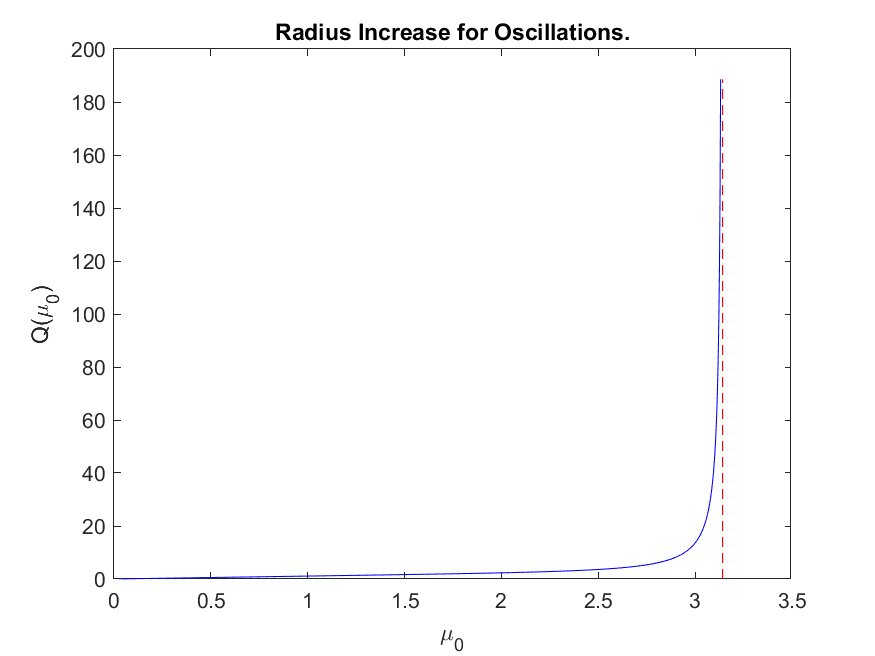
\includegraphics[width=0.5\textwidth]{images/Qmu.png}
    \caption{The plot of \(Q(\mu_0)\).}
    \label{fig:acrobot-Q}
\end{figure}

We can therefore state that, for each \(\mu_0 \in \, ]0,\pi[\), there exists
\(I\) such that
\[
    P_\mathcal{O}(\mu_0) = \mu_0\left(1+ IKQ(\mu_0)\right) + R(\pi,\mu_0,I) > 0
    .
\]
Unfortunately, Khalil's perturbation theory does not guarantee this \(I\) is the
same for all \(\mu_0\). 

We deal with this issue by taking the compact set
\[
    \bar{\mathcal{O}} := \left\{(q_u,p_u) \in \Gamma 
    \mid E(q_u,p_u) \leq E(\pi,0) \right\}
    .
\]
The remainder term \(R(\pi,\mu_0,I)\) is smooth and of order \(I^2\),
which means it can be written in the form 
\(R(\pi,\mu_0,I) = I^2\tilde{R}(\mu_0,I)\)
for some \(\tilde{R}\) a smooth function.
Since \(\bar{O}\) is compact, \(\tilde{R}\) attains its minimum
\(\underbar{r}\) on \(\bar{O}\).
Hence, \(R(\pi,\mu_0,I)\) is bounded below by the parabola
\(\underbar{r}I^2\), which means
\begin{equation}\label{eqn:acrobot-Po-lowerbound}
    P_\mathcal{O}(\mu_0) \geq \mu_0\left(1 + IKQ(\mu_0)\right) + I^2\underbar{r}
    .
\end{equation}
Because \(I\) is assumed to be small, the term \(I^2\) shrinks rapidly.
If \(\underbar{r} < 0\), we can find a value of \(I\) which overcomes
the effect of \(I^2\underbar{r}\) and make \(P_\mathcal{O}\) positive.
Furthermore, ~\eqref{eqn:acrobot-Po-lowerbound} implies that, for fixed \(I\),
\(P_\mathcal{O}(\mu_0)\) is monotonically increasing in \(\mu_0\).

We conclude that, for all \(m\), \(g\), \(l\), \(\bar{q}_a\), and for
any \(\epsilon > 0\), there exists \(I(\epsilon)\) small enough so that
the Poincar\'{e} section \(P_\mathcal{O}(\mu_0)\) is positive for all
\(\mu_0 \in ]\epsilon,\pi[\) and 
\(\lim \limits_{\mu_0 \to \pi} P_\mathcal{O}(\mu_0) = \infty\).

\subsection*{Energy gain on \(\mathcal{O}_\epsilon\)}
To simplify notation, denote by \(x(t) := (q_u(t),p_u(t))\) the orbit of the
acrobot with initial condition \(x(0)\).
Let \(\epsilon > 0\) and define
\[
    \mathcal{O}_\epsilon := \left\{(q_u,p_u) \in \Gamma
    \mid E(\epsilon,0) < E(q_u,p_u) < E(\pi,0)\right\}
    ,
\]
with \(\bar{\mathcal{O}}_\epsilon\) its (compact) closure.

Since \(\bar{\mathcal{O}}_\epsilon \subset \mathcal{O}\), we still have 
\(\dot{\alpha} > 0\), which means \(x(t)\) spirals clockwise around the origin.
If this orbit remains in \(\mathcal{O}\), it must intersect
the \(q_u\) axis at some radius \(\mu = \delta\)
which depends on the initial condition \(x(0)\).
Take 
\[
    \underbar{\delta} = 
    \min\limits_{x(0) \in \bar{\mathcal{O}}_\epsilon} \delta(x(0))
    ,
\] 
which exists because \(\bar{\mathcal{O}}_\epsilon\) is compact.
From the previous perturbation analysis,
there exists \(I\) small enough that \(P_\mathcal{O}(\mu_0)\) 
is positive for all \(\mu_0 \in ]\underbar{\delta},\pi[\).

Suppose \(x(0) \in \mathcal{O}_\epsilon\), and the orbit
intersects the \(q_u\)-axis at some point \(x(t_0) = (m_0, 0)\).
The Poincar\'{e} section \(P_\mathcal{O}(|m_0|)\) is positive because 
\(|m_0| > \underbar{\delta}\).
As the acrobot continues its oscillation, it might exit
\(\mathcal{O}\) if it has gained enough energy;
if not, it will intersect the \(q_u\) axis again at
a new point \(x(t_1) = (m_1,0)\).
Theorem \ref{thm:khalil-perturbation} guarantees that \(|m_1|\) differs
from \(P_\mathcal{O}(|m_0|)\) only up to order \(I^2\), 
which means \(|m_1| > |m_0|\).
From here, we can apply Theorem \ref{thm:khalil-perturbation} iteratively:
initializing the acrobot at \(x(t_i) = (m_i, 0)\), the
next intersection with the \(q_u\) axis will be at
\(x(t_{i+1}) = (m_{i+1},0)\) with \(|m_{i+1}| > |m_i|\).

Because the Poincar\'{e} section is monotonically increasing, 
the orbit will eventually reach an intersection point \(x(t_N) = (m_N,0)\)
such that \(P_\mathcal{O}(|m_N|) > \pi\). 
At this point, the orbit will no longer return to the
\(q_u\)-axis.
Instead, it will escape \(\mathcal{O}\) entirely; 
in doing so, it also escapes \(\mathcal{O}_\epsilon\).
Hence, the orbit must escape any compact subset of \(\mathcal{O}\) in finite
time, which means the acrobot is gaining energy on \(\mathcal{O}_\epsilon\).

Setting \(I < 0\), the Poincar\'{e} section \(P_\mathcal{O}(\mu_0)\) is now
decreasing.
Hence, the orbit in \(\mathcal{O}_\epsilon\) spirals clockwise towards the origin, 
which means the constraint is dissipating energy.

% Empty proof environment to put QED square on the right of the page
\begin{proof}[\unskip\nopunct]
\end{proof}

\subsection*{Perturbation Analysis for Rotations}
The rotation region for the nominal pendulum is the set
\[
    \mathcal{R} := \left\{ (q_u,p_u) \in \Gamma \mid E(q_u,p_u) > E(\pi,0)\right\}
    .
\]
We wish to find a new set of coordinates \((\beta,\rho)\) for the acrobot
and perform a similar analysis to what we did for oscillations.
In the oscillation region \(\mathcal{O}\) we showed that the nominal pendulum's
energy (and hence, its orbit) is uniquely determined by the intersection point
\(\mu\) with the \(q_u\)-axis; 
when the nominal pendulum is rotating, the energy is instead determined by the
intersection \(\rho\) on the \(p_u\)-axis.
Note that the boundary of \(\mathcal{O}\) intersects the \(p_u\) axis when 
\(p_u^2 = 60m^2 g l^3\); 
hence, for a rotation we must have \(\rho > \sqrt{60 m^2 g l^3}\) if the
orbit has momentum \(p_u > 0\) 
or \(\rho < -\sqrt{60 m^2 g l^3}\) if the orbit has momentum \(p_u < 0\).
The energy level set associated with \(\rho\) is
\[
    \left\{(q_u,p_u) \in \Gamma \mid E(q_u,p_u) = \frac{\rho^2}{10ml^2}\right\}
    ,
\]
which gives the relationship
\begin{equation}\label{eqn:rotation-pu2}
    \frac{p_u^2}{10m l^2} + 30mgl(1 - c_u) = \frac{\rho^2}{10 ml^2}
    .
\end{equation}
On this level set, \(q_u\) takes all values on \(\Sone\), so our angle of
rotation is uniquely parameterized by \(\beta = q_u\).
Since \(\rho\) does not change sign along the rotation, we have the smooth
relationship
\begin{align}\label{eqn:rotation-Tinv}
    q_u &= \beta
    , \\
    p_u &= \sign{\rho}\sqrt{\rho^2 - 30 m^2 g l^3\left(1 - c_\beta \right)}
    .
\end{align}

Inverting this relationship gives our (smooth) transformation
\begin{equation*}
    T : \SxR \rightarrow 
    \Sone \times ]-\infty,-60m^2gl^3[\, \cup \, ]60m^2gl^3,\infty[ 
    ,
\end{equation*}
where \(T(q_u,p_u) = (\beta,\rho)\) is defined by
\begin{align}\label{eqn:rotation-T}
    \beta &= q_u
    , \\
    \rho &= \sign{p_u}\sqrt{p_u^2 + 30 m^2 g l^3 \left(1 - c_u \right)}
    .
\end{align}

Computing the acrobot's constrained dynamics in \((\beta,\rho)\)-coordinates and
setting \(I = 0\) yields the dynamics of the nominal pendulum.
MATLAB evaluates those dynamics as
\begin{align}\label{eqn:acrobot-rot-mu-dot-nom}
    \dot{\rho}_n &= 0
    , \\
    \label{eqn:acrobot-rot-alpha-dot-nom}
    \dot{\beta}_n &=  \sign{\rho} 
    \frac{\sqrt{\rho^2 - 30m^2gl^3(1 - c_\beta)}}{5ml^2}
    .
\end{align}
As expected, \(\dot{\beta}_n\) does not change sign on \(\mathcal{R}\) because
a rotating pendulum does not change direction:
if \(\rho_n > 0\), the orbit traces a curve going from \(\beta_n = -\pi\) to 
\(\beta_n = \pi\); if \(\rho_n < 0\) the curve goes in the reverse direction.
By continuity of the acrobot's constrained dynamics 
\((\dot{\beta},\dot{\rho})\), we must also have 
\(\sign{\dot{\beta}} = \sign{\rho_0}\) for small enough \(I\).
Hence, we can use \(\beta\) as a new ``time" variable on \(\mathcal{R}\) 
by performing a time transformation \(t = \tau(\beta)\).
This produces the time-scaled system \(\hat{\rho}(\beta) = \rho(\tau(\beta))\)
with dynamics
\[
    \begin{cases}
        \dot{\hat{\rho}} = \frac{\dot{\rho}}{\dot{\beta}}
        , \\
        \hat{\rho}(0) = \rho_0
        .
    \end{cases}
\]
For a perturbation approach, be expand the solution of these dynamics into
\begin{equation}\label{eqn:acrobot-rhohat-approx}
    \hat{\rho}(\beta,\rho_0,I) = \hat{\rho}_0(\beta,\rho_0) + I
    \hat{\rho}_1(\beta,\rho_0) + R(\beta,\rho_0,I)
    ,
\end{equation}
where \(R(\beta,\rho_0,I)\) is \(O(I^2)\).

From ~\eqref{eqn:khalil-perturbation-nominal} we know
\(\hat{\rho}_0\) is the solution to the nominal system
\[
    \begin{cases} 
        \dot{\hat{\rho}}_0 = 0
        , \\
        \hat{\mu}_0(0) = \rho_0
        ,
    \end{cases}
\]
which means \(\hat{\mu}_0(\beta,\rho_0) \equiv \rho_0\) for all \(\beta\).
Likewise, ~\eqref{eqn:khalil-perturbation-firstorder} 
gives us the following dynamics for \(\hat{\rho}_1\):
\begin{equation}\label{eqn:acrobot-rho1-dot}
  \begin{cases}
    \dot{\hat{\rho}}_1 =
    \frac{5m^2 g l^3 \bar{q}_a \left(
        m^2gl^3\left(18s_\beta^2 + 30c_\beta(1 - c_\beta)\right)
        - c_\beta\rho_0^2
    \right)}{
    |\rho_0|\sqrt{\rho_0^2 - 30m^2gl^3(1 - c_\beta)}
    }
    =: b(\beta,\rho_0)
     , \\
     \hat{\rho}_1(0) = 0
     .
 \end{cases}
\end{equation}
The solution to ~\eqref{eqn:acrobot-rho1-dot} is given by
\[
    \hat{\rho}_1(\beta,\rho_0) = \int \limits_0^\beta b(\sigma,\rho_0)d\sigma
    .
\]

Supposing we initialize the acrobot at \((\beta,\rho) = (0,\rho_0)\),
then one full rotation amounts to \(\beta\) traversing \(2\pi\)rad in a clockwise
direction (\ie \(\beta\) going from \(0\) to \(\sign{\rho_0}2\pi\)).
We define a Poincar\'{e} section as the point reached on the \(p_u\) axis after
every rotation:
\[
    P_\mathcal{R}(\rho_0) = \rho_0 + I \hat{\rho}_1(\sign{\rho_0}2\pi, \rho_0)
      + R(2\pi,I)
    .
\]
If \(|P_\mathcal{R}(\rho_0)| > |\rho_0|\), then the rotation has
driven the orbit further from the origin.
In other words, \(|p_u|\) has increased across the rotation.
If this is true for any \(\rho_0\), the acrobot is gaining momentum, which in
turn means it is gaining energy.

The function \(b(\beta,\rho_0)\) is even in both its inputs, and is 
\(2\pi\)-periodic in \(\beta\).
Hence, we have 
\begin{align*}
    \hat{\rho}_1(\sign{\rho_0}2\pi, \rho_0) &=
    \int \limits_0^{\sign{\rho_0}2\pi} b(\sigma,\rho_0)d\sigma
    , \\
     &=\sign{\rho_0}\int\limits_0^{2\pi}b(\sigma,\rho_0)d\sigma
     , \\
     &= \sign{\rho_0} \hat{\rho}_1(2\pi,\rho_0)
     .
\end{align*}
Furthermore, \(\hat{\rho}_1(2\pi,\rho_0) = \hat{\rho}_1(2\pi,|\rho_0|)\).
This implies that
\[
    |P_\mathcal{R}(\rho_0)| = \left|\sign{\rho_0}\left(
        |\rho_0| + I \hat{\rho}_1(2\pi,|\rho_0|)\right)
    \right|
    = P_\mathcal{R}(|\rho_0|)
    .
\]
Hence, if \(P_\mathcal{R}(|\rho_0|) > |\rho_0|\) (or equivalently if
\(\hat{\rho}_1(2\pi,|\rho_0|) > 0\))
the phase \((q_u(t),p_u(t))\) initialized at \((0,\rho_0)\) 
will intersect the \(p_u\) axis at a point \(p > \rho_0\).
If we could guarantee that \(\hat{\rho}_1(2\pi,\rho_0) > 0\)
for all \(\rho_0 > \sqrt{60m^2gl^3}\), then the acrobot would be spiraling away
from the origin on \(\mathcal{R}\).

Unfortunately, we cannot adimensionalize
\(b(\beta,\rho_0)\) like we did for oscillations. 
Using the assumption , we have that 
\(\hat{\rho}_1(2\pi,\rho_0) > 0 \) for all 
\(\rho_0 \in ]\sqrt{60m^2gl^3},\rho_0[\).
We conclude that, for small enough \(I\), the Poincar\'{e} section 
\(P_\mathcal{R}(\rho_0)\) is monotonically increasing when 
\(0 < \rho_0 < \bar{\rho}\) and
monotonically decreasing when \(-\bar{\rho} < \rho_0 < 0\).  

\subsection*{Energy Gain on \(\Omega\)}
We will prove the acrobot gains energy on the set 
\[
    \Omega := \left\{ (q_u,p_u) \in \Gamma 
     \mid E(q_u,p_u) < E(0,\bar{\rho}) \right\}
    .
\]
% Can we use the jacobian? The spectrum is hard to find.
% TODO: W and D's boundary is two elements: the point (pi,0) and the curve of the
% homoclinic orbit connecting (pi,0) to (-pi,0). We need to show that almost
% every initial condition starting in \(mathcal{O}\) will NOT converge to (pi,0), and
% therefore exit D and enter W.

Define the set of points in \(\mathcal{R}\) which have pseudo-radius in \(U\) by
\[
    W := \left\{(q_u,p_u) \in \Gamma \mid |\rho(q_u,p_u)| \in U \right\}
    ,
\]
as in Figure \ref{fig:acrobot-rot-W}.
Monotonicity of \(P(\rho_0)\) means there are no closed orbits of 
\((q_u,p_u)\) on \(W\). 
Furthermore, \(|p_u|\) is increasing every time the orbit hits the
\(p_u\)-axis. 

\begin{figure}
    \centering
    % TODO: Display the set W, which is the two rotation bands at the top and
    % bottom with outer limit +- \bar{mu}  and inner limit +- sqrt{60m^2gl^3}.
    % Show also that the inner limit connects to D
    %\includestandalone[width=0.5\textwidth]{images/acrobot_rot_W}
    \caption{The set \(W\) of points which have pseudo-radius 
        \(|\rho| \in ]\sqrt{60m^2gl^3}, \bar{\rho}[\). The inner boundary of \(W\)
        is \((q_u,p_u) = (\pi,0)\), which is also the boundary of the
        oscillation domain \(mathcal{O}\).}
    \label{fig:acrobot-rot-W}
\end{figure}

We conclude that \(|\rho(q_u,p_u)|\) will eventually reach \(\bar{\rho}\). 
We cannot claim this fits the definition  of energy injection 
(since \((0,0) \notin W\)), but we can still say that \((q_u,p_u)\) will
eventually depart \(W\) through the outer boundary in finite time.
The acrobot is thereby gaining energy in the literal sense that its momentum
is increasing on \(W\).

If we set \(I < 0\), we have \(P(|\rho_0|) < |\rho_0|\).
Hence, \(|p_u|\) is decreasing every time the orbit hits the \(p_u\)-axis, so
the acrobot will eventually depart \(W\) through the inner boundary. 
The acrobot is losing momentum, and therefore it is losing energy on \(W\).

A hybrid supervisor that flips the sign of \(I\) based on the current
value of \(\mu\) will stabilize any energy level of oscillation.
As was the case in the VLP, this supervisor should implement some kind of
hysteresis to avoid infinite switching.


\section{Experimental Results}
% TODO: This might be a separate chapter

%/========== /Acrobot ==========/%
% vim: set tw=80 ts=4 sw=4 sts=0 et ffs=unix :
